\documentclass[10pt,handout]{beamer}

\usepackage[french]{babel}
\usepackage[T1]{fontenc}
\usepackage[utf8]{inputenc}
\usepackage[
    left = \flqq{},%
    right = \frqq{},%
    leftsub = \flq{},%
    rightsub = \frq{} %
]{dirtytalk} 	% for \say{}
\usepackage{xcolor} 	% for color text
\usepackage{csquotes}
\usepackage{amssymb}
\usepackage{mathtools}
\usepackage{array}

\usetheme{Frankfurt}
\usetheme{CambridgeUS}
\usetheme{JuanLesPins}
%\usetheme{Montpellier}
%\usetheme{Madrid}

\usecolortheme{dolphin}

\useinnertheme{circles}
\usefonttheme{structurebold}
\useoutertheme{default}

%\hypersetup{pdfpagemode=FullScreen}

\title[Chemins spécifiques]{Chemins spécifiques pour la classification dans les réseaux de neurones profonds}
\author[Bouzidi, Elhouiti, Kezzoul, Zeroual, Dadi]{Bouzidi Belkacem - Dadi Mélissa \\ Elhouiti Chakib - Kezzoul Massili \\ Zeroual Ramzi}
\institute[]{Université de Montpellier}
\date{\today}

% Pour inserer une frame de sommaire avant chaque debut de section
\AtBeginSection[]
{
  \placelogofalse
  \begin{frame}
    \tableofcontents[hideothersubsections,currentsection,subsectionstyle=show/shaded/hide]
  \end{frame}
  \placelogotrue
}

% Mettre les listes en triangle
\setbeamertemplate{itemize item}[triangle]

%Insertion d'un logo
\newif\ifplacelogo % create a new conditional
\placelogotrue % set it to true
\logo{\ifplacelogo
\includegraphics[height=12mm]{img/univ-montpellier.png}\fi}

%------------------------------------------------------%
% page de titre
%------------------------------------------------------%
\begin{document}

\placelogofalse
\begin{frame}
	\titlepage
\end{frame}

\placelogotrue

\section{Introduction}
\subsection{Les réseaux de neurones profonds}

\placelogofalse 
\subsection{Le jeu de données}
\begin{frame}{MNIST}
    \makebox[\textwidth]{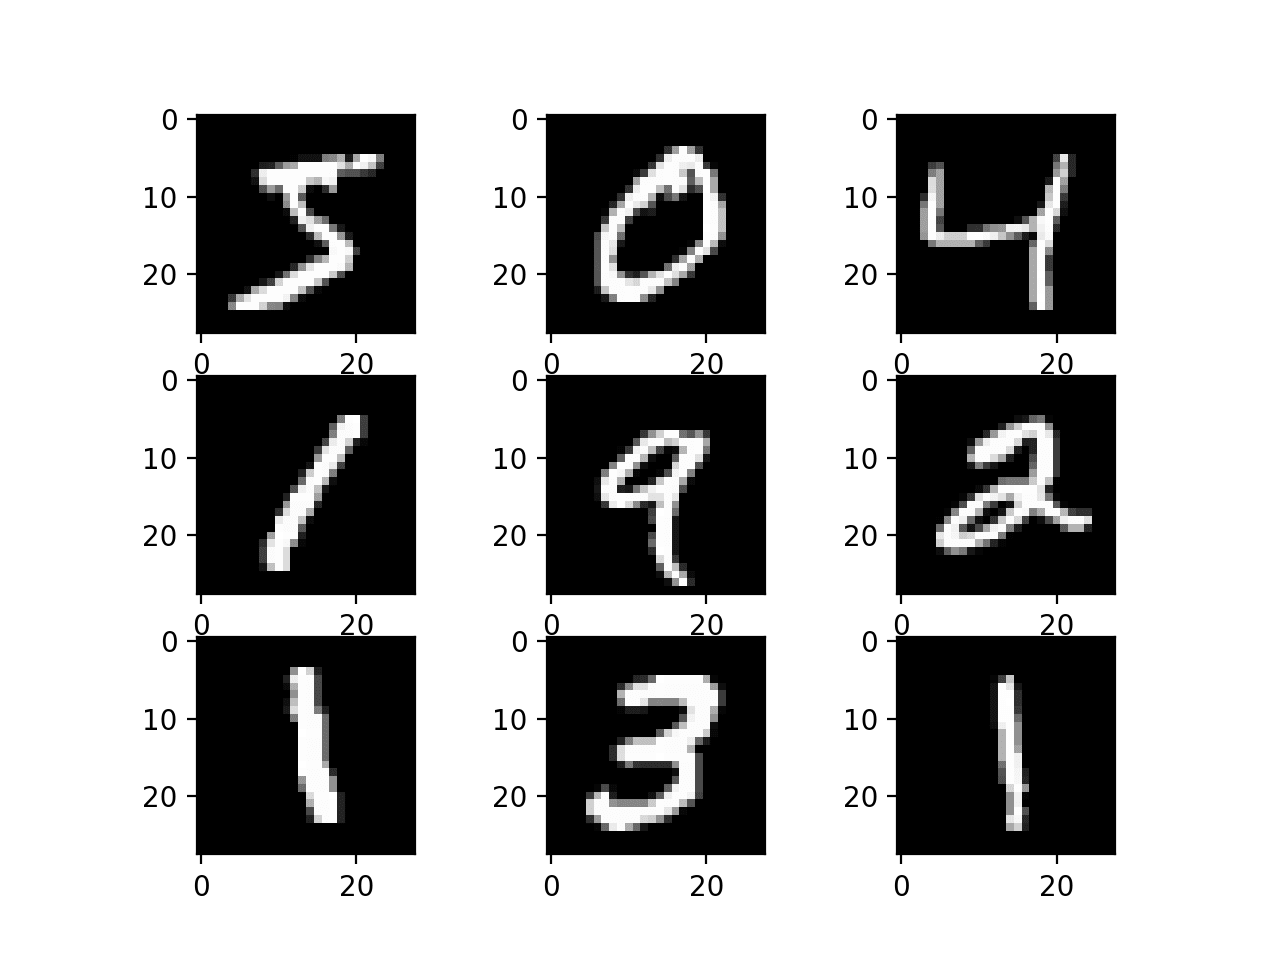
\includegraphics[width=0.8\textwidth]{img/mnist.png}}
\end{frame}
\placelogotrue

\placelogofalse 
\subsection{Problèmatique}
\begin{frame}{Problèmatique}
    \begin{block}{Boite noire}
        Les réseaux de neurones semblent s'appliquent à la manière d'une boite noire. Aucune information n'est fournie sur ce qui les a conduits à atteindre leurs prédictions.
    \end{block}
    \begin{block}{Objectifs}
        L'objectif est de comprendre le fonctionnement interne d'un réseau de neurones et de repérer des signatures d'activation de neurones en variant les données.
    \end{block}

    \makebox[\textwidth]{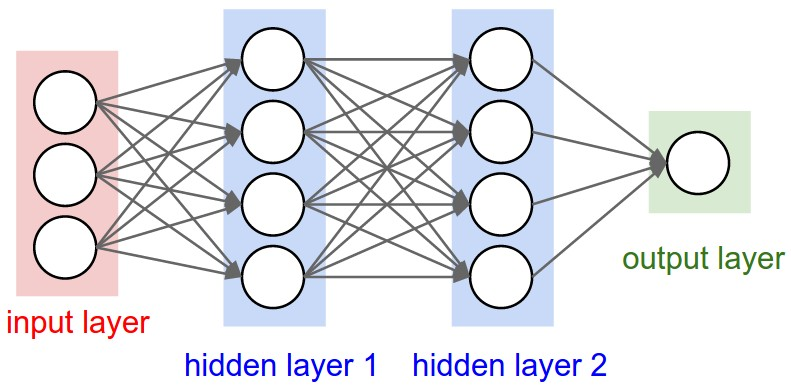
\includegraphics[width=0.6\textwidth]{img/ann-dense.jpg}}
        
\end{frame}
\placelogotrue

\begin{frame}{Questions qu'on se posent}
    Par exemple, si on entraîne un modèle à reconnaître des images de 1 et de 7
    \begin{itemize}
        \item À partir de quelle couche le modèle change de comportement pour reconnaître une image ?
        \item Les signatures des images de \textit{7}, sont-elles différentes de ceux des \textit{1} ?
        \item Si on passe une image de \textit{3} au modèle, à quoi va ressembler sa signature ?
    \end{itemize}    
\end{frame}

\subsection{Solution proposée}
\begin{frame}{Solution proposée}
    \begin{itemize}
        \item Construire des réseaux de neurones.
        \item Récupérer, pour chaque donnée, la sortie des couches cachées.
        \item Extraire les signatures grâce à des algorithmes de \textit{clustering}.
        \item Réaliser une interface de visualisation en utilisant différentes techniques.
        \item Analyser les résultats et répondre aux questions.
    \end{itemize}
\end{frame}

\section{Organisation}

\section{Analyse des données}
\subsection{Découpage des données}
\subsection{Prétraitement}

\section{Développement de l’architecture}
\subsection{Technologies utilisées}
\subsection{Modèle d'apprentissage}
\subsection{Signature et Clustering}
\subsection{Interface de visualisation}

\section{Analyse des résultats}
\subsection{Réponse aux questions}
\subsection{Conclusion}

\begin{frame}
    \begin{center}
      Merci pour votre attention.
    \end{center}
\end{frame}
  
\end{document}